%!TEX root = ../thesis.tex
%*******************************************************************************
%****************************** Second Chapter *********************************
%*******************************************************************************

\chapter{Continuous model}

\ifpdf
    \graphicspath{{Chapter2/Figs/Raster/}{Chapter2/Figs/PDF/}{Chapter2/Figs/}}
\else
    \graphicspath{{Chapter2/Figs/Vector/}{Chapter2/Figs/}}
\fi

Sheets of \textit{C. flexa}, despite being discretely made up of individual cells, appear to take on curvature when looked at as a whole. In an effort to avoid the complexity of tracking a cell-cell connection network, I approximated sheets of \textit{C. flexa} with continuous surfaces. 

I begin by developing a one-dimensional filament model with inversion dynamics, which demonstrates that azimuthal stretching is key to understanding the flipping process observed in \citet{brunet2019}. I proceed to describe a method for approximating sheets of \textit{C. flexa} with two-dimensional surfaces and relate the collar-opening angle $\phi$ and collar-collar contact angle $\psi$ to surface curvature. I write an expression for the sheet energy and vary it to derive a shape equation.

\section{One-dimensional model} \label{sec:c_1d}

We are interested in the problem of \textit{Choaneca flexa} inversion. For intuition, suppose we have a one dimensional filament with position $\vec{r}(s)$ parameterised by arclength $s$. If the filament has prescribed curvature $\kappa_0$, then the bending energy functional $\varepsilon$ is given by 

\begin{align}
    \varepsilon[\vec{r}(s)] &= \frac{1}{2} A \int (\kappa - \kappa_0)^2 ds, \nonumber \\
    \intertext{where the curvature $\kappa$ is deduced from $\vec{r}(s)$ and $A$ is the bending modulus. If the filament is short relative to the characteristic bending length scale, we express the problem in the Mange representation by writing $\vec{r}(s) = (x, h(x))$ for a height function $h(x)$. The resulting energy is written in terms of the prescribed (signed) curvature $H_0$, } \nonumber \\
    \varepsilon[\vec{h}(x)] &= \frac{1}{2} A \int_0^L (h_{xx} - H_0)^2 dx. \label{eq:energy}
\end{align}

We postulate that the filament experiences isotropic drag with coefficient $\zeta$ in a viscous medium, with the dynamics are described by a functional derivative of the energy:

\begin{align}
    \zeta \vec{r}_t &= -\frac{\delta \varepsilon}{\delta \vec{r}} \nonumber \\
    \zeta h_t &= -\frac{\delta \varepsilon}{\delta h}. \label{eq:eom} \\
    \intertext{Taking the functional derivative of equation \ref{eq:energy}, we find the energy change} \nonumber \\
    \delta \varepsilon &= \left. A(h_{xx} - H_0)\delta h_x \right|_0^L - \left. Ah_{3x} \delta h \right|_0^L + A \int h_{4x} \delta h ds \label{eq:func_deriv} \\
    \intertext{in terms of the boundary conditions of $h$.}
\end{align}

If we take free-end boundary conditions $h_{xx}(0, L) = 0 = h_{3x}(0, L)$, the boundary terms in equation \ref{eq:func_deriv} vanish and we are left with the equation of motion 

\begin{align}
    \zeta h_t &= -A h_{4x} \label{eq:eom_mange}
\end{align}

We nondimensionalise equation \ref{eq:eom_mange} by re-expressing $x$ as $x/L$ and $t$ as $t / (\frac{\zeta L^4}{A})$ (the labels $x, t, h, H_0$ are left unchanged for readability) to derive $h_t = -h_{4x}$ with boundary conditions $h_{xx}(0, 1) = 0 = h_{3x}(0, L)$. It is clear that the ground state of equation \ref{eq:energy} is given by a quadratic height function with quadratic term $\frac{1}{2}H_0x^2$. Let $h_*(x) = -\frac{1}{2} H_0(x-\frac{1}{2})^2 + \frac{1}{8}H_0$ be one such ground state, and suppose $h(x, 0) = -h_*(x)$. Note that the filament in $h(x, 0)$ is not in the ground state since the curvature is given by $H_0$. 

The dynamics of the displacement $g(x, t) = h(x, t) - h_*(x)$ is given by $g_t = g_{4x}$. If $g(x, t) = e^{-\sigma t} f(x)$ for some $f(x)$ and eigenvalue $\sigma$, we obtain the ordinary boundary value problem 

\begin{align}
    \frac{d^4f}{dx^4} &= \sigma f & \begin{cases} f''(0, 1) = 0 \\ f'''(0, 1) = 0. \end{cases} \label{eq:bvp}
\end{align}

It is clear that the general solution of $f$ is $A \sin kx + B \cos kx + D \sinh kx + E \cosh kx$. As in BPFD 4.2.3, the derivatives $f''(0) = f'''(0) = 0$ gives $A = D, B = E$. Moreover, the eigenvalues $\sigma = k^4$ are given by the sequence of solutions $k_n$ to 

\begin{align}
    \cos k - \frac{1}{\cosh k} &= 0. \label{eq:roots}
\end{align}

Equation \ref{eq:roots} is plotted in Figure \ref{subfig:roots} along with the positions of the solutions $k_n$ as solved numerically. The solution $k_0 = 0$ is omitted because it contributes a constant term to $h(x, t)$ that does not evolve in time. The eigenfunctions $w_n(x)$ with eigenvalues $k_n^4$ are normalized on the interval $[0,1]$ numerically, and the ratio $A/B$ is given by $(\sinh k - \sin(k)) / (\cosh k - \cos k)$. The first five eigenfunctions are shown in Figure \ref{subfig:efuncs}. 

\begin{figure}[tbhp]
    \centering
    \begin{subfigure}[b]{0.48\textwidth}
        \centering
        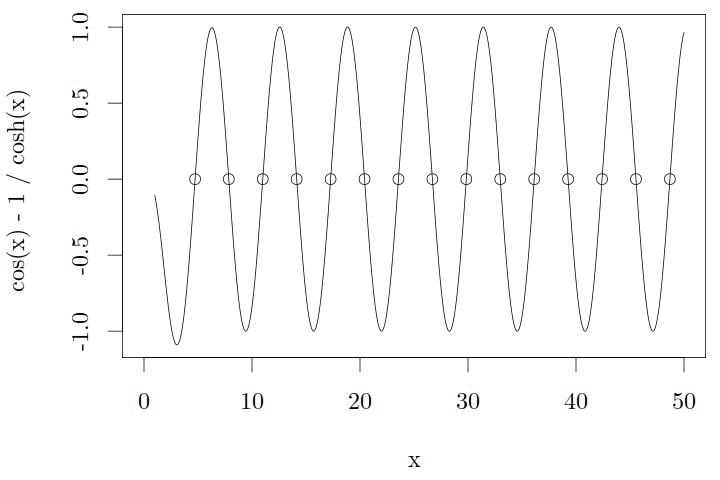
\includegraphics[width=\textwidth]{eq_roots.png}
        \caption{Equation \ref{eq:roots} and its solutions.}
        \label{subfig:roots}
    \end{subfigure}
    ~
    \begin{subfigure}[b]{0.48\textwidth}
        \centering
        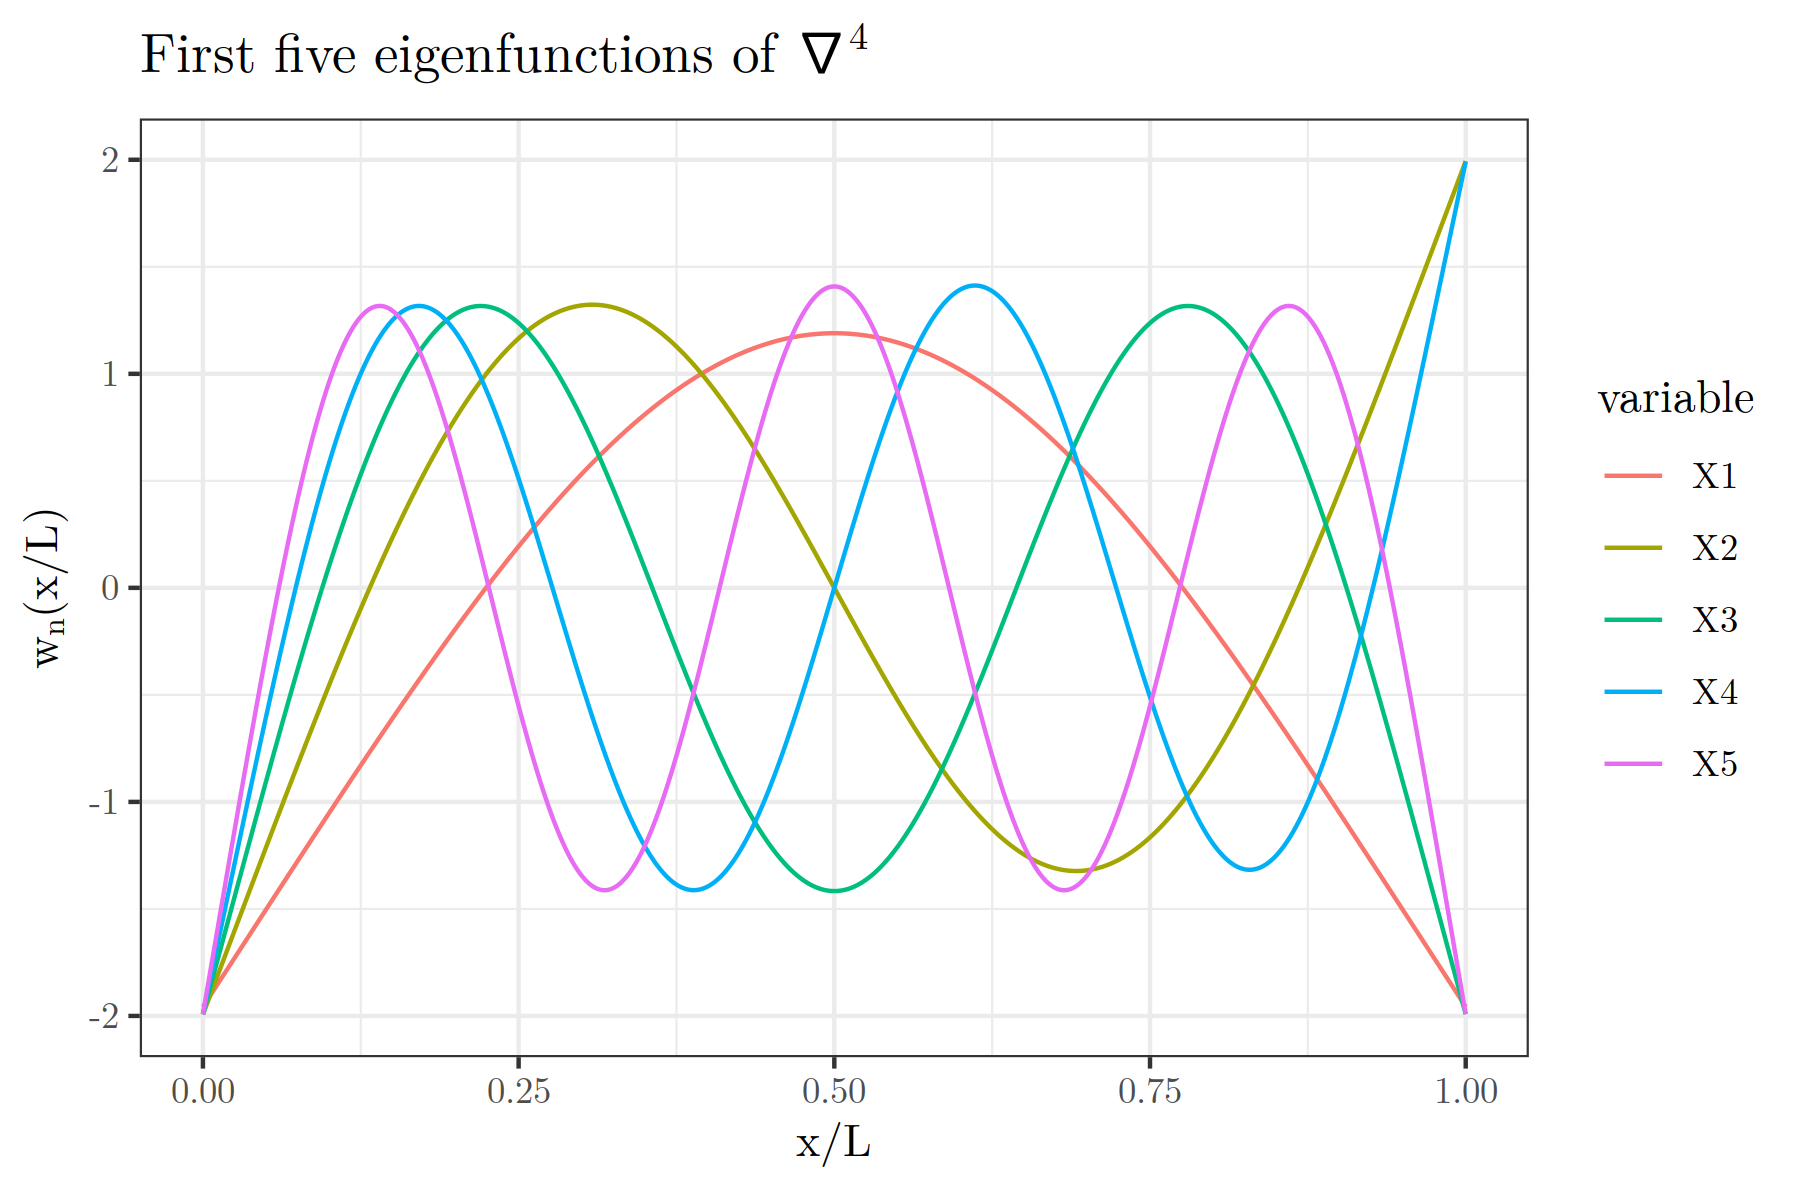
\includegraphics[width=\textwidth]{efuncs.png}
        \caption{The first five eigenfunctions $f_n$ of boundary value problem \ref{eq:bvp}.}
        \label{subfig:efuncs}
    \end{subfigure}
    \caption{Solving the boundary value problem in equation \ref{eq:bvp}}
    \label{fig:bvp_sol}
\end{figure}

Letting $f(x) = \sum_{n=1}^\infty a_n f_n(x)$, we get that $a_n = \int_0^1 g(x, 0) f_n(x)dx$, and the complete dynamics of the height function are given by 

\begin{align}
    h(x, t) &= h_*(x) + g(x) = h_*(x) + \sum_{n=1}^\infty a_n e^{k_n^4 t} f_n(x). \label{eq:sol}
\end{align}

\noindent In practice, only the solutions $k_n$ to equation \ref{eq:roots} shown in Figure \ref{subfig:roots} are used, since the approximation to $h(x, 0)$ is close and higher $k_n$ result in precision errors when calculating $\cosh kx$ and $\sinh kx$. 

For the initial conditions given previously, the time evolution of $h(x, t)$ is shown in Figure \ref{fig:shapes}. We can make a few observations:

\begin{itemize}
    \item The system evolves extremely quickly in non-dimensional time. This is because each mode's evolution is given by rate $k_n^4$, which grows rapidly and makes higher order terms negligible almost immediately. Maybe it is worth asking what the values of the bending modulus and drag coefficient are to see if the timescale $\zeta L^4 / A$ is very large to compensate.
    \item The time evolution slows at larger $t$. This makes sense as the change in energy $\delta \varepsilon$ becomes smaller in magnitude when the curvature $h_{xx}(x, t)$ becomes closer to that of $h_*(x, t)$.
    \item We see some ``rolling inward'' of the change in curvature from the outer edge, most clearly at $t = \num{9e-4}$. However, it does not seem as pronounced as in \textit{C. flexa} inversion, at least not to me. When the organism inverts, it seems to have a wave of flipping that moves from the edge towards the center. Perhaps this is because the \textit{C. flexa} collars are stiff such that they resist compression or stretching in the sheet. Our representation used here does not penalize the filament compressing, which it clearly does as its arclength decreases substantially during the transition. 
\end{itemize}

\begin{figure}[bthp]
    \centering
    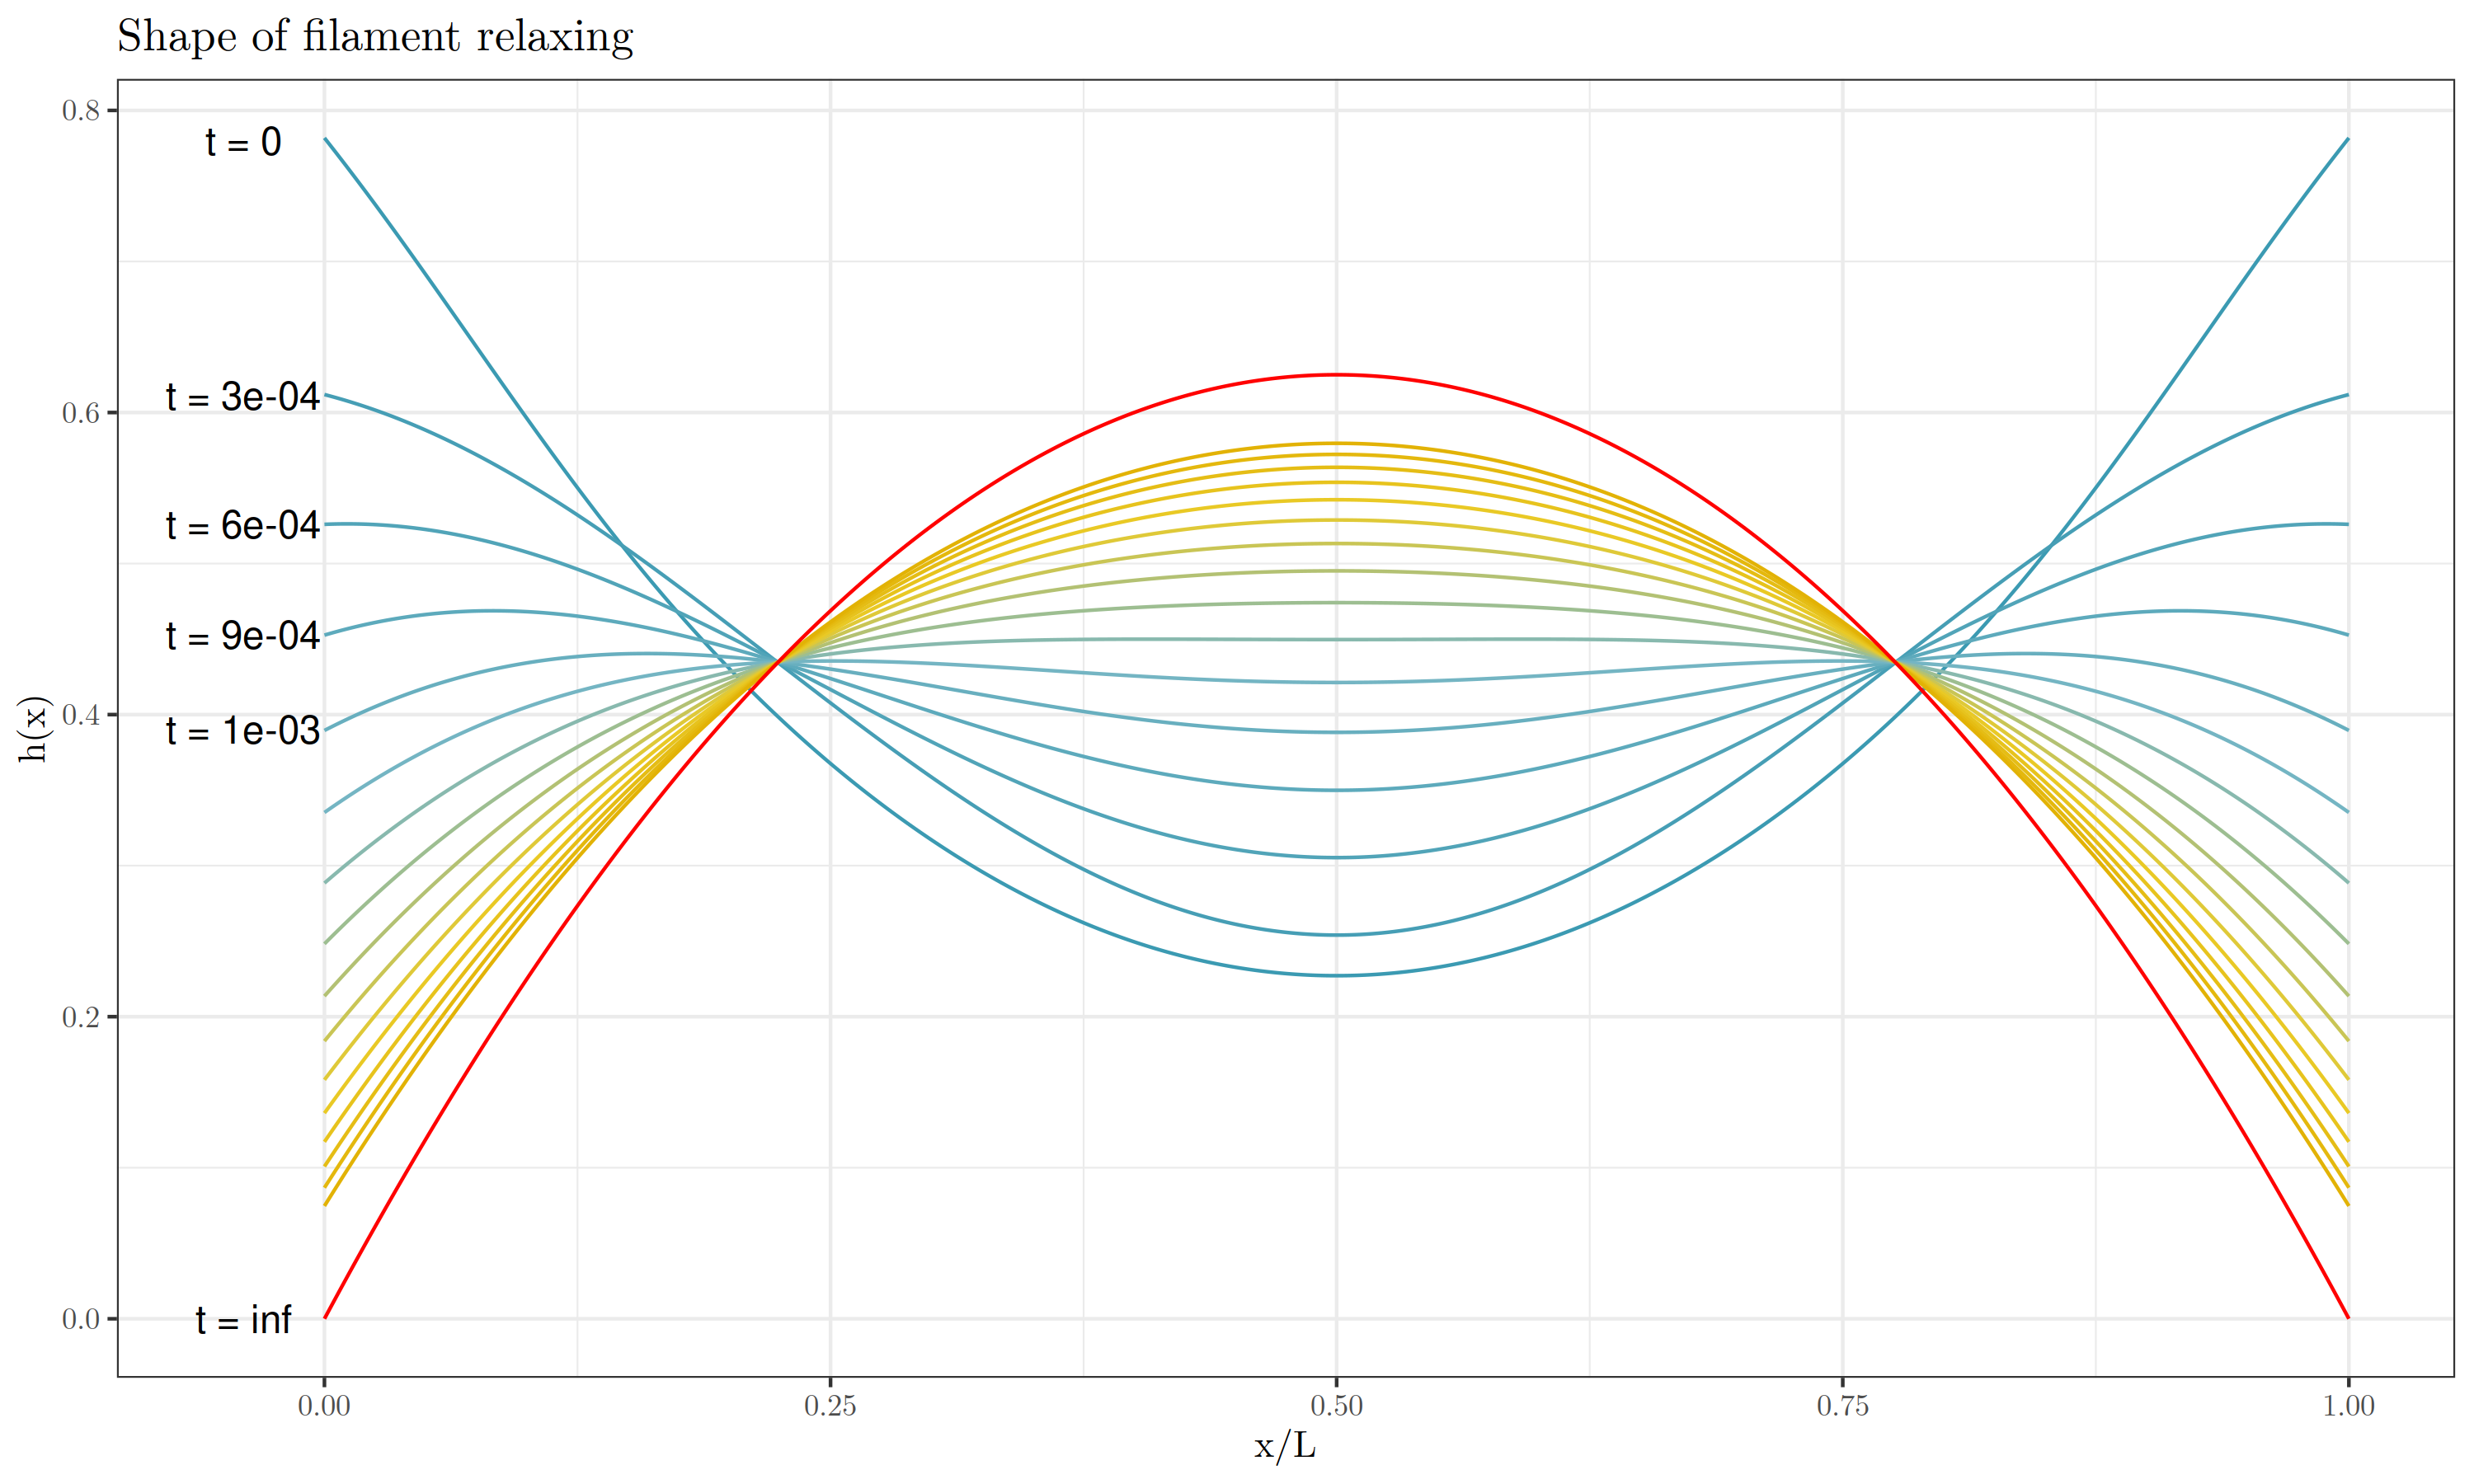
\includegraphics[width=\textwidth]{shapes.png}
    \caption{Time evolution of a one-dimensional filament which switches prescribed curvature sign instantaneously. Time and length are given in dimensionless units defined by the length $L$, bending modulus $A$, and drag coefficient $\zeta$. The time unlabeled time intervals continue sequentially in intervals of $\Delta t = \num{3e-4}$.}
    \label{fig:shapes}
\end{figure}

\section{Surface approximation}

The simplified dynamics that we get from the Mange representation lack energetic costs from the compression and extension that come with deforming a two dimensional surface. The logical step to include these energies is to model the flexa sheet a surface of revolution based on a curve $\bm{r}(\rho, \theta)=(\rho \cos \theta, \rho \sin \theta, z(\rho))$ with cylindrical coordinates $\rho, \theta$ and height function $z$. In doing so, we could take the elastohydrodynamic equation of motion written in terms of curvature $H$ and $K$ and express it as purely as a function of $z$.

We will proceed by writing the equations of motion generally for a surface and reducing it to a surface of revolution.

\subsection{$H$ and collar connection angle}

Before getting into the continuous sheet problem, it is worth describing the two degrees of freedom that our collar connections afford. The collar makes an angle $\phi$ between the vector pointing directly out of the cell and the vector between the cell and its collar boundary with the next cell. Additionally, there is an angle between the collars of two adjacent cells $\psi$. The latter results in the sheet's curvature, so we want to relate it to mean curvature $H$ or preferred curvature $H_0$. 

\begin{figure}[htbp]
    \centering
    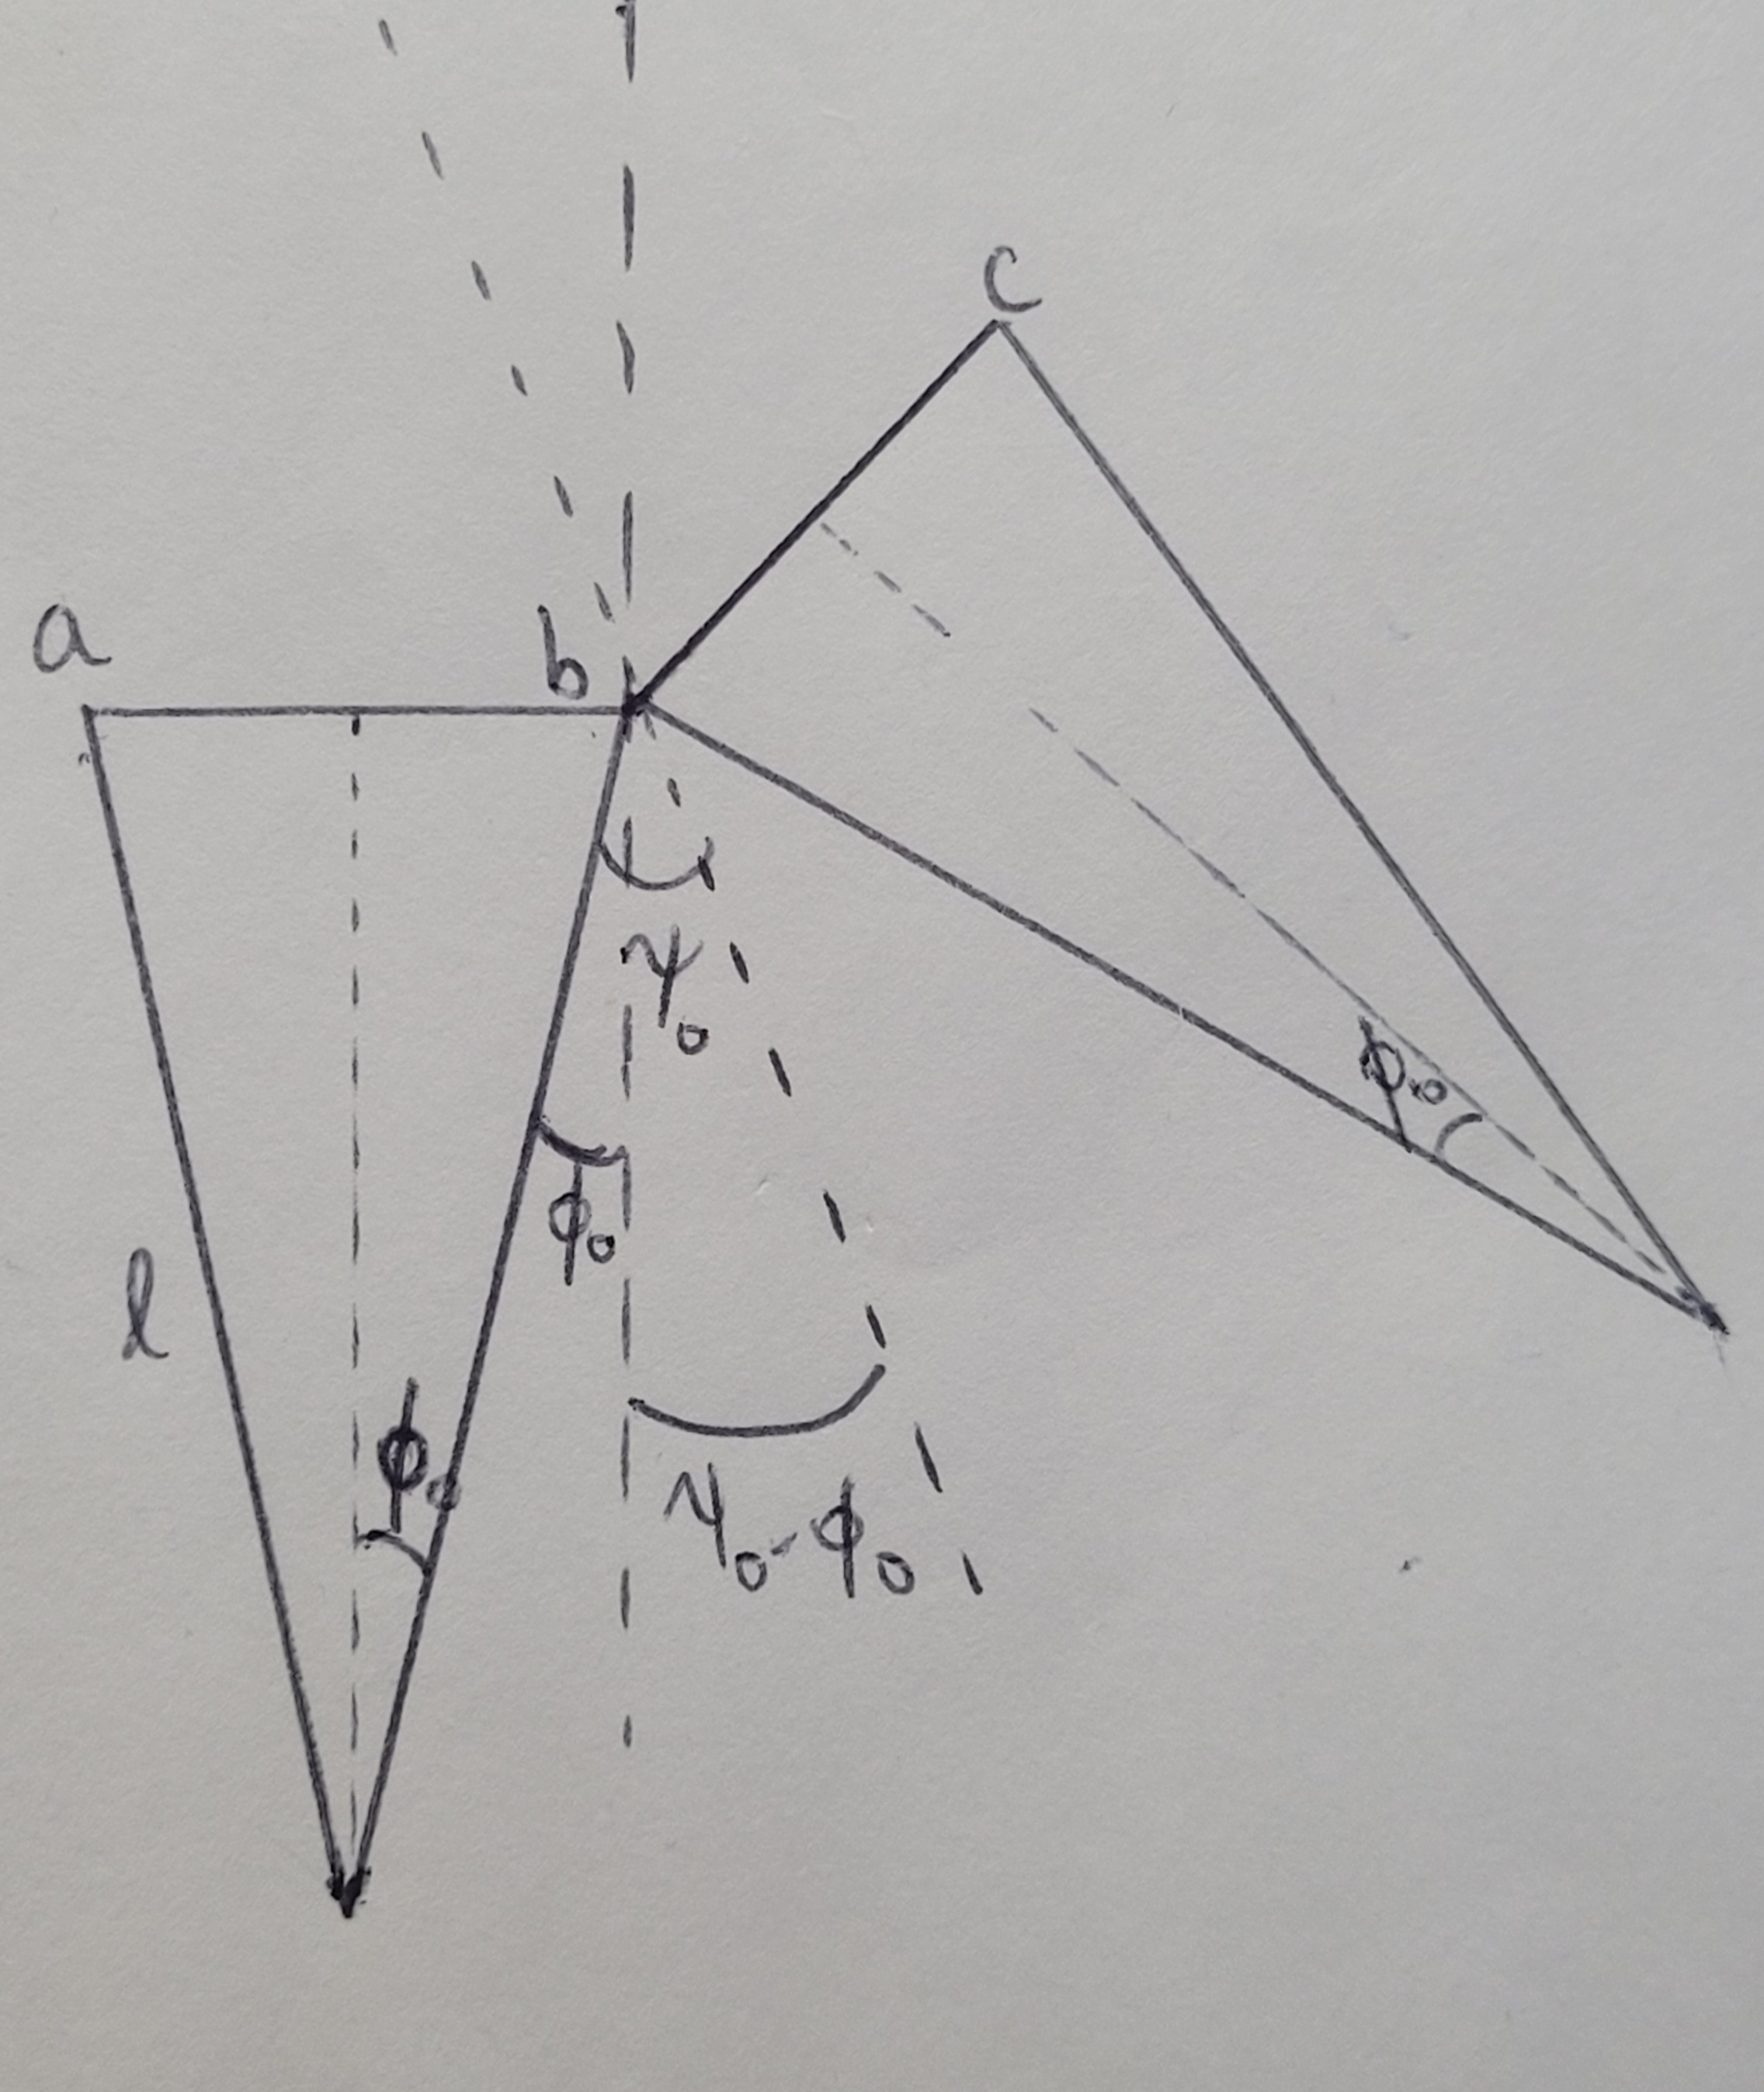
\includegraphics[width=0.5\textwidth]{hpsi.jpg}
    \caption{Geometry for relating collar boundary angle $\psi$ to curvature $H$. }
    \label{fig:hpsi}
\end{figure}

Consider two neighboring cells with collar boundaries $a$, $b$, and $c$, as shown in Figure \ref{fig:hpsi}. We might imagine defining a radius of curvature by the circle that passes through the three collar boundaries. If we set $\bm{x_a} = 2\ell\sin\phi_0(-1, 0)$, $\bm{x_b} = (0,0)$, and $\bm{x_c} = 2\ell\sin\phi_0 (\sin(\psi_0 - \phi_0), \cos(\psi_0-\phi_0)$, we can solve for the circle coordinates 

\begin{align*}
    (x_\circ, y_\circ) &= \ell \sin\phi_0\left(-1, \frac{1+\cos2(\psi_0 - \phi_0)}{\sin2(\psi_0 - \phi_0)} \right)
\end{align*}

\noindent to get the inverse radius of curvature 

\begin{align}
    H_0 = \frac{1}{\sqrt{x_\circ^2 + y_\circ^2}} &= \frac{\sin(\psi_0 - \phi_0)}{\ell \sin\phi_0}. 
\end{align}

This has a nice, simple interpretation in that if $\psi_0 > \phi_0$, $H_0 > 0$ (as drawn in Figure \ref{fig:hpsi}). On the other hand, $\psi_0 < \phi_0$ implies $H_0 < 0$, or the sheet is concave on the cell body side. 

Alternatively, we solve for $\psi_0$ as a function of $H_0$,

\begin{align}
    \psi_0 &= \phi_0 + \arcsin \left( H_0 \ell \sin \phi_0 \right). \label{eq:h0_psi}
\end{align}

As we find later in equation \ref{eq:hlb}, the curvature of the sheet in any given direction is greater than or equal to $-1/\ell$ (cell bodies and collars cannot go through each other). This lower bound corresponds in \ref{eq:h0_psi} to $\psi_0 = 0$, which we expect when cells are pressing tightly against each other (Figure \ref{fig:maxcurv}).


\subsection{Problem statement} \label{subsec:problem}

\citet{powers2010} (Section IV.B) shows that for an energy density $\e$ written in terms of the first and second fundamental forms $g_{\alpha\beta}$ and $K_{\alpha\beta}$, we can write an expression for the stress tensor $\bm{F}^\alpha$ 

\begin{align}
    \bm{F}^\alpha &= \left(T^{\alpha\beta} + \e^{\alpha\beta}K_\gamma^\beta \right)\bm{t}_\beta - (\nabla_\beta \e^{\alpha\beta})\hat{\bm{n}}. \label{eq:stress}
\end{align}

\noindent Here, $K_\gamma^\beta = K_{\gamma \delta}g^{\delta \beta}$, $\bm{t}_\beta = \partial_\beta \bm{r}$, and 

\begin{align*}
    T^{\alpha\beta} &= g^{\alpha\beta} \e + 2 \frac{\partial \e}{\partial g_{\alpha\beta}} = \frac{2}{\sqrt{g}} \frac{\partial}{\partial g_{\alpha\beta}} \left(\sqrt{g}\e \right) \\
    \e^{\alpha\beta} &= \frac{\partial \e}{\partial K_{\alpha\beta}}
\end{align*}

\noindent with $g = \det{g_{\alpha\beta}}$.

Since the force $\bm{f}$ acting on a surface point is given by the covariant divergence of the stress $\nabla_\alpha \bm{F}^\alpha$, our problem is effectively solved once we decide on an appropriate energy density. \citet{brunet2019} showed that the angle formed by the \textit{C. flexa} collars changes when individual cells are triggered for inversion. We might reasonably suggest preferred sheet curvature is prescribed by changing the preferred angle of the collar $\phi_0$ and imposing and energetic cost based on the amount that the collar angle $\phi(\theta)$ differs around the collar in $\theta$: $\e \sim \int (\phi(\theta) - \phi_0)^2 d\theta$.

\subsection{Connecting continuous surface with individual cell mechanics}

For any point on a smooth surface, we could find an orthonormal basis of eigenvectors $\bm{e}_1, \bm{e}_2$ in the tangent space that diagonalises $K_\mu^\nu$. In terms of a vector $\bm{\Delta \xi}$ written in this basis, we have that the change in height with respect to the tangent plane and its normal $\Delta h$ is given by $K_{\mu\nu}\Delta\xi^\mu\Delta\xi^\nu$.

Let's consider a cell with collar angle $\phi(\theta)$, where $\theta$ measures the location on the collar. If the cell has an optimal collar angle $\phi_0$ and corresponding optimal curvature $K_{0\mu\nu}$, then the height of the collar will be $K_{0\mu\nu}\Delta\xi_0^\mu\Delta\xi_0^\nu$. The distance from the centerline of the cell (the norm of $\bm{\Delta\xi_0}$) is determined by $\phi_0$. The geometry is shown in Figure \ref{fig:geom}.

\begin{figure}[htbp]
    \centering
    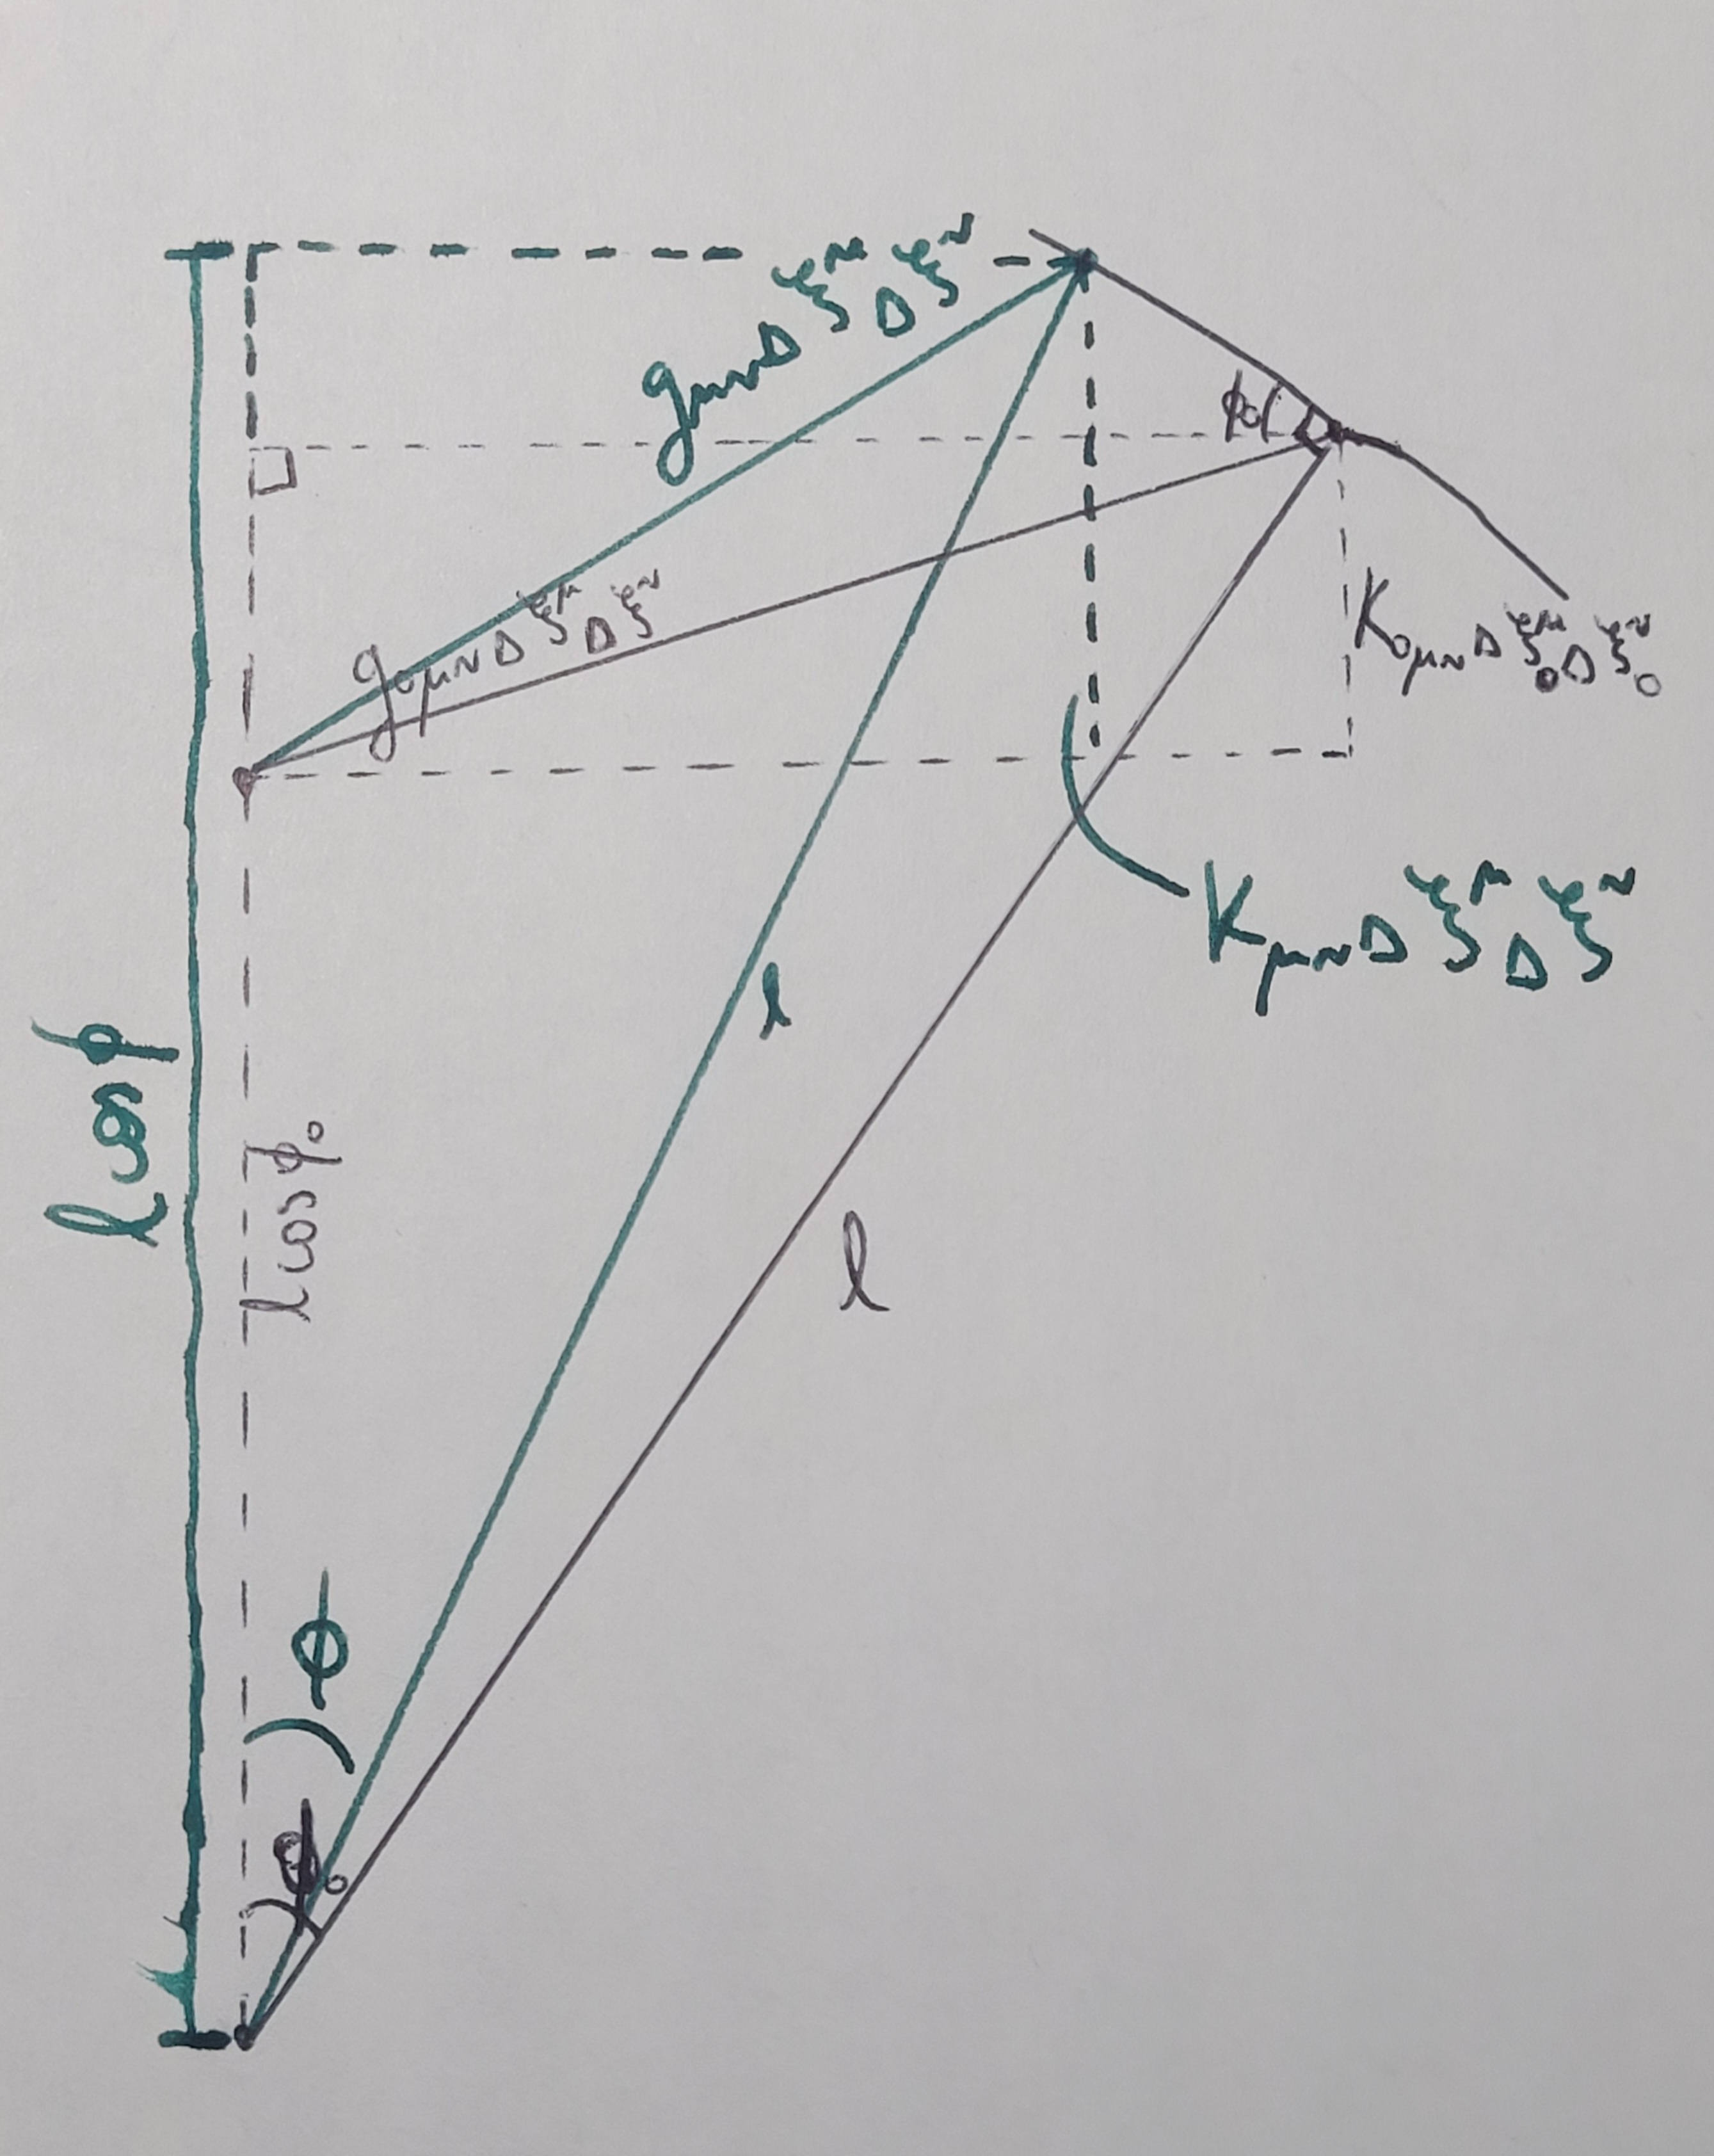
\includegraphics[width=0.75\textwidth]{geom.jpg}
    \caption{Geometry of a single cell and collar with a continuous surface approximating the interactions between collars.}
    \label{fig:geom}
\end{figure}

If the cell has collar angle $\phi$ in direction $\theta$, we know the collar distance as $\bm{\Delta\xi} = \ell(\cos\phi, \sin\phi)$. For a fixed collar length $\ell$, we know the difference in height between the ground state and deformed state is $\ell(\cos\phi - \cos\phi_0)$. We can then relate the collar angle and sheet curvature by equating 

\begin{align}
    K_{\mu\nu}\Delta\xi^\mu\Delta\xi^\nu - K_{0\mu\nu}\Delta\xi_0^\mu\Delta\xi_0^\nu &= \ell(\cos\phi - \cos\phi_0). \label{eq:base}
\end{align}

The radius out from the center for the ground state is $\ell\sin\phi_0$ while for the deformed state it is $\ell\sin\phi$, so for $K_{011}=K_{022}=H_0$, we get

\begin{align*}
    K_{\mu\nu}\ell^2\sin^2\phi (\cos\theta, \sin\theta)^{\mu,\nu} - H_0 \ell^2\sin^2\phi_0 &= \ell(\cos\phi - \cos\phi_0) \\
    H_\theta \ell^2\sin^2\phi - H_0 \ell^2\sin^2\phi_0 &= \ell(\cos\phi - \cos\phi_0)
\end{align*}

\noindent where $H_\theta = K_{11}\cos^2\theta + K_{22}\sin^2\theta + 2K_{12}\sin\theta\cos\theta$ is the curvature of a line on the surface in direction $\theta$. We can cancel a factor of $\ell$, redefine units of length in terms of $\ell$ (such that $H_\theta$ is the ratio of $\ell$ with the radius of curvature in direction $\theta$), and express $\sin^2\phi$ in terms of $\cos\phi$ to get

\begin{align*}
    0 &= H_\theta \cos^2\phi + \cos\phi + (H_0\sin^2\phi_0 - \cos\phi_0 - H_\theta) \\
    \cos\phi &= \frac{-1 \pm \sqrt{1 + 4H_\theta (H_\theta + \cos\phi_0 - H_0\sin^2\phi_0)}}{2H_\theta}.
\end{align*}

If we take the collars to always have angle $0 \leq \phi \leq \pi/2$, we can constrain $0 \leq \cos\phi \leq 1$ to find the two inequalities 

\begin{align}
    H_\theta \geq H_0 \sin^2\phi_0 - \cos\phi_0 \label{eq:ineq1}\\
    1 \geq \cos\phi_0 - H_0 \sin^2\phi_0. \label{eq:ineq2}
\end{align}

\noindent The second inequality can be simplified to $H_0 \geq -(1+\cos\phi_0)^{-1}$. Combining the two inequalities yields 

\begin{align}
    H_\theta \geq -1. \label{eq:hlb}
\end{align}

\noindent Re-expressed with units, this means that $H_\theta \geq -1/\ell$, or that the radius of curvature can never be smaller than $\ell$ on the cells' side. In other words, the cells can't push through each other! (Figure \ref{fig:maxcurv})

\begin{figure}[hbtp]
    \centering
    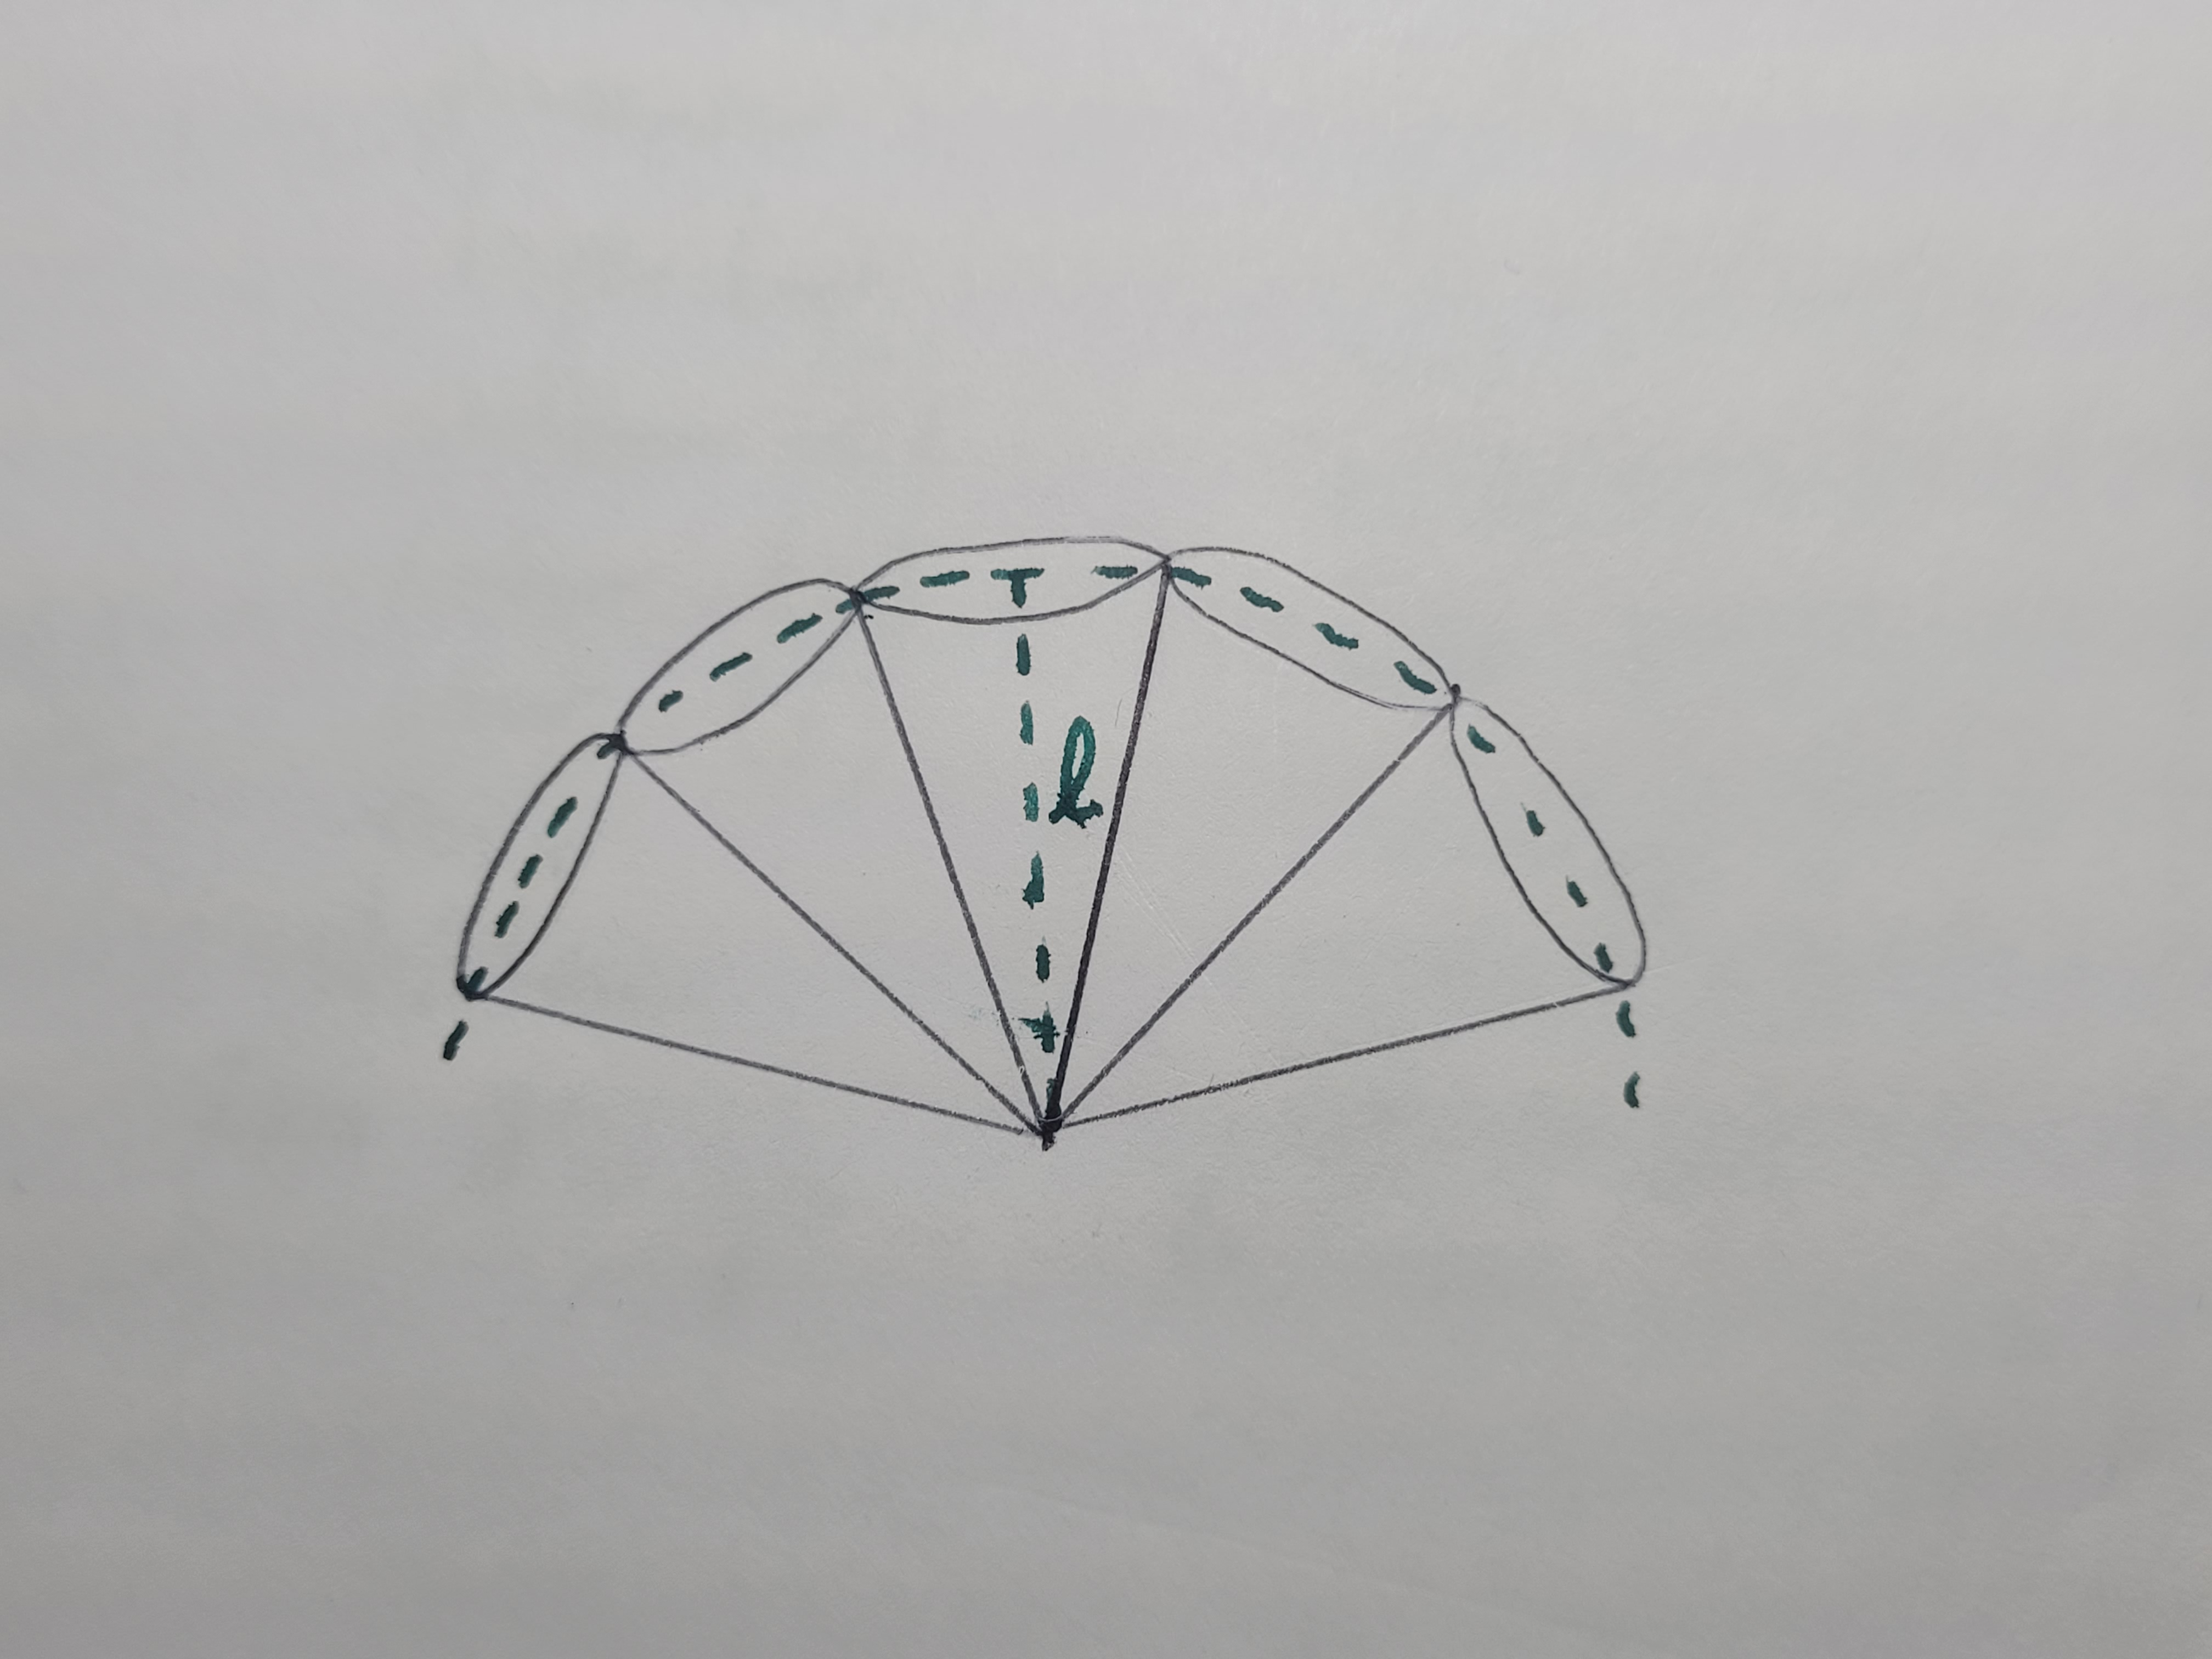
\includegraphics[width=0.5\textwidth]{arc.jpg}
    \caption{Maximum cell-side curvature is given by inequalities \ref{eq:ineq1}, \ref{eq:ineq2} to have radius $\ell$. This corresponds to every (point) cell bumping into each other.}
    \label{fig:maxcurv}
\end{figure}

\subsection{Writing the energy}

We want to write equation \ref{eq:base} in terms of $\phi-\phi_0$ to write down the energy. We can use a trigonometric identity to write

\begin{align}
    H_\theta \sin^2\phi - H_0 \sin^2\phi_0 &= -2 \sin \frac{\phi - \phi_0}{2} \sin\frac{\phi + \phi_0}{2}. \label{eq:preapprox}
\end{align}

\noindent If $phi - phi_0$ is small in magnitude, then 

\begin{align*}
    \sin\frac{\phi - \phi_0}{2} &\approx \frac{\phi - \phi_0}{2} \\
    \sin\frac{\phi + \phi_0}{2} = \sin\left(\phi_0 + \frac{\phi + \phi_0}{2} \right) &\approx \sin\phi_0 + \frac{\phi - \phi_0}{2} \cos\phi_0 \\
    \sin^2\phi = \sin^2\left(\phi_0 + (\phi - \phi_0) \right) &\approx \sin^2\phi_0 +(\phi - \phi_0)\sin2\phi_0.
\end{align*}

Using these approximations we rewrite equation \ref{eq:preapprox} to first order in $\phi - \phi_0$ as

\begin{align*}
    (H_\theta - H_0) \sin^2\phi_0 + H_\theta (\phi - \phi_0)\sin2\phi_0 &= -(\phi - \phi_0) \sin\phi_0 \\
    (H_\theta - H_0) \sin^2\phi_0 &= -(\phi-\phi_0) (H_\theta \sin2\phi_0 + \sin\phi_0) \\
    \frac{(H_\theta-H_0)^2 \sin^4\phi_0}{(H_\theta + \sin\phi_0 / \sin2\phi_0)^2 \sin^2 2\phi_0} &= (\phi - \phi_0)^2.
\end{align*}

We want to integrate this function in $\theta$, so let $K_{11} = a$, $K_{22} = b$, $K_{12} = c$, $-H_0 = d$ and $\sin\phi_0/ \sin 2 \phi_0 = e$ for simplicity when we write

\begin{align*}
    \int_{-\pi}^\pi (\phi - \phi_0)^2 d\theta &= \int_{-\pi}^\pi \frac{\left(a\cos^2\theta + b\sin^2\theta + 2c\sin\theta\cos\theta + d \right)^2}{\left(a\cos^2\theta + b\sin^2\theta + 2c\sin\theta\cos\theta + e \right)^2} d\theta \\
    &= \left\{-\sin2\theta \left[a^2 (-4bc\theta -4ce\theta + d^2 - 2de +e^2) + a(4b^2c\theta -2b(d-e)^2+4c\theta(c^2 - e^2)) \right. \right. \\
    &\qquad \qquad \qquad \left. + b^2(4ce\theta + d^2 -2de + e^2) + 4bc\theta(e^2 - c^2) + 4c^2 (d-e)^2 \right] \\
    &\qquad + 2(a + b +2e) \left[c^2 \theta (b - a) + \theta (a - b) (a + e) (b + e) - c (d - e)^2 \right] \\
    &\qquad \left.+ 2 \theta (a - b)^2 \cos(2 \theta) (a (b + e) + e (b + e) - c^2) \right\} \\
    &\qquad \big/ 2\left[(a - b) (a (b + e) + e (b + e) - c^2) ((a - b) \cos(2 \theta) + a + b + 2 c \sin(2 \theta) + 2 e)\right] \\
    &\quad + \frac{(e - d) (a (4 b + d + 3 e) + b d + 3 b e - 4 c^2 + 2 d e + 2 e^2) \tan^{-1}\left(\frac{-(b + e) \tan\theta - c}{\sqrt{a (b + e) + e (b + e) - c^2}}\right)}{2(a (b + e) + e (b + e) - c^2)^{3/2}}
\end{align*}

\noindent evaluated at $\theta = -\pi, \pi$. Evaluating this expression is surprisingly straightforward, and gives the result 

\begin{align*}
    \int_{-\pi}^\pi (\phi - \phi_0)^2 d\theta &= \text{const.} + \text{const.} \frac{4 K + 2(d+3e)H + 2de + e^2}{(K + 2H + e^2)^{3/2}}.
\end{align*}

Varying this expression will be more difficult than the typical membrane energy defined only in terms of curvature $(H-H_0)^2 + K$ since the Gaussian curvature term is not alone. This means that we cannot use the Gauss Bonnet theorem $\int_S K dA = 2\pi n + \oint_{\partial S}K ds$ to simply write it as a boundary term. Nevertheless, provided that we can vary $K$ on the surface, the shape equation that results shouldn't be very difficult to derive.

\subsection{Varying the energy}

Following subsection \ref{subsec:problem}, we just need to express our energy in terms of $K_{\mu\nu}$ and $g_{\mu\nu}$ to derive a force from it. We of course have that $H = (1/2) (K_{\mu\nu} g^{\mu\nu})$, which is easily differentiated with respect to $K_{\mu\nu}$ and $g_{\mu\nu}$. We can differentiate $K$ by re-expressing it with the identity $K^{\alpha\beta}K_{\alpha\beta} = 4H^2 - 2K$.\footnote{This comes from $4H^2 - 2K = (K^1_1 + K^2_2)^2 - 2(K^1_1K^2_2 - 2K^1_2) = (K^1_1)^2 + 2 K^1_2K^1_2 + (K^2_2)^2 = K^\alpha_\beta K_\alpha^\beta = K^{\alpha\beta}K_{\alpha\beta}$.} Then we have $K = (g^{\alpha\beta}K_{\alpha\beta})^2 - K_{\mu\nu}K_{\alpha\beta}g^{\mu\alpha}g^{\nu\beta}$.

\section{Energy variation}


